\begin{figure}[!t]
  \centering
  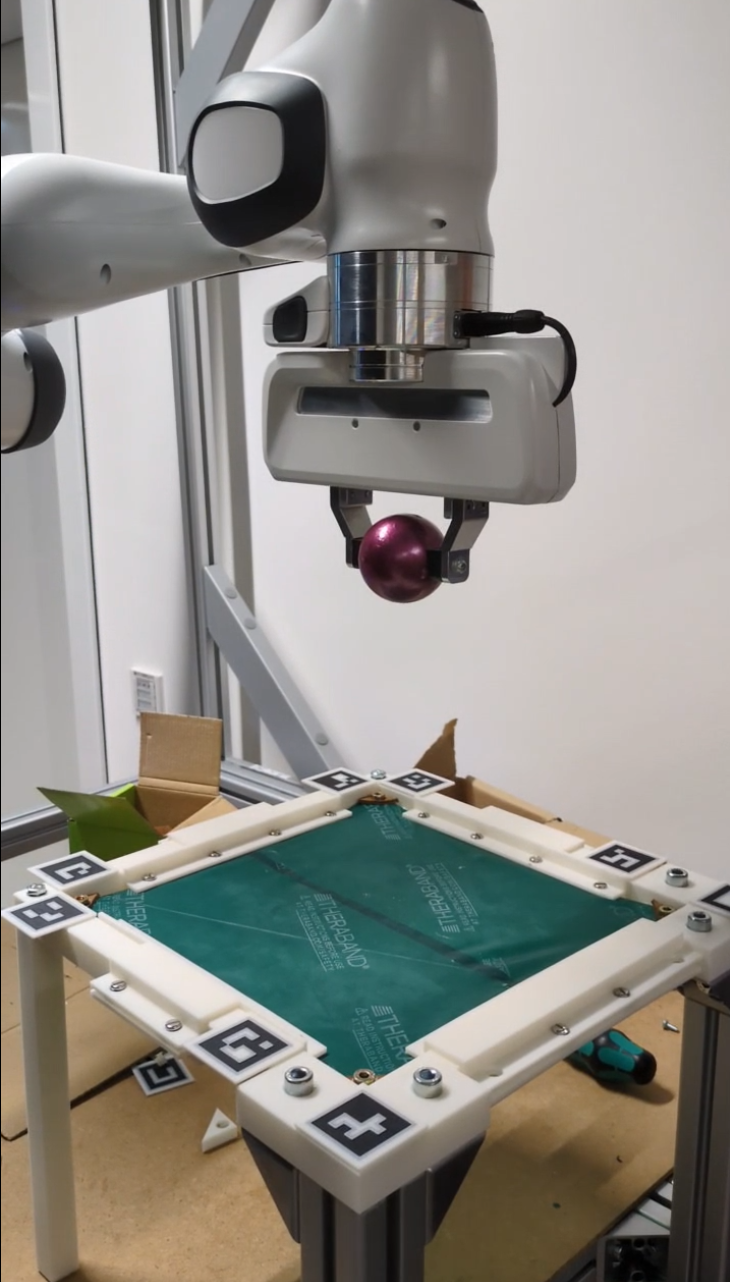
\includegraphics[width=0.192\textwidth, trim={0 2.5cm 0 3.5cm}, clip]{figures/qualitative_realworld_data/01.png}\hfill
  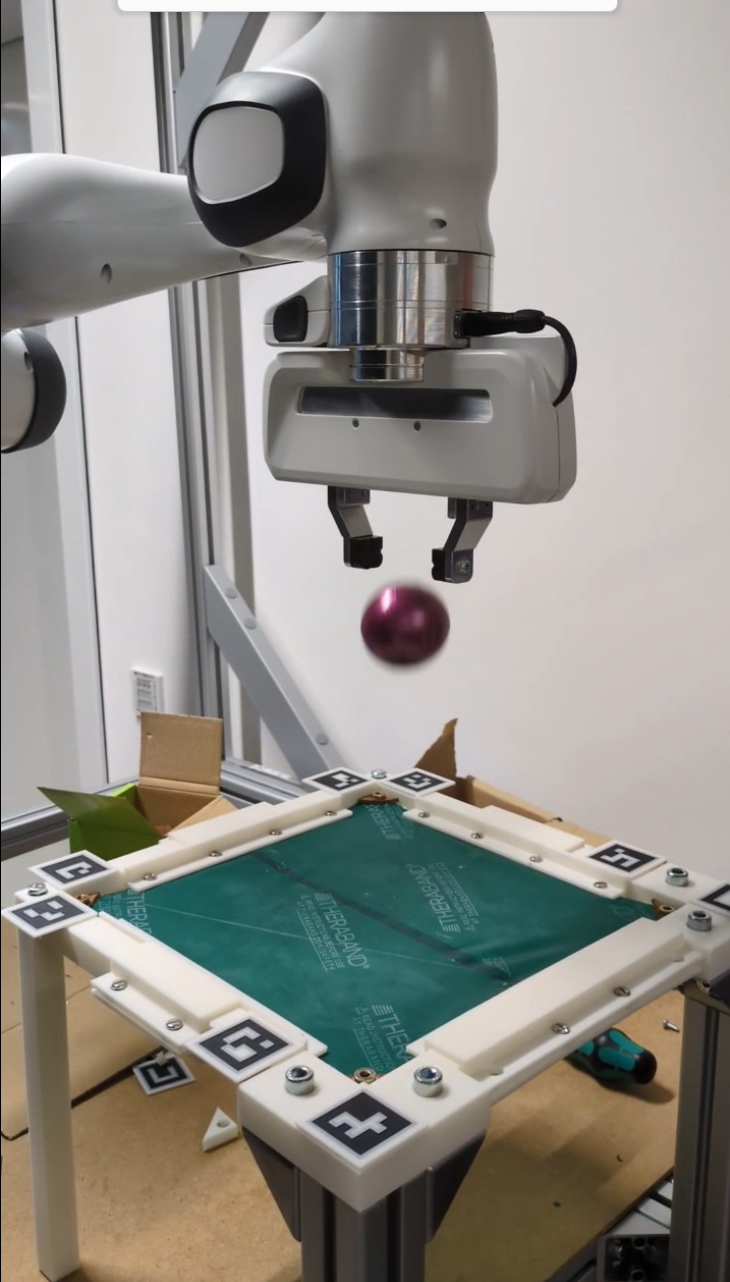
\includegraphics[width=0.192\textwidth, trim={0 2.5cm 0 3.5cm}, clip]{figures/qualitative_realworld_data/02.png}\hfill
  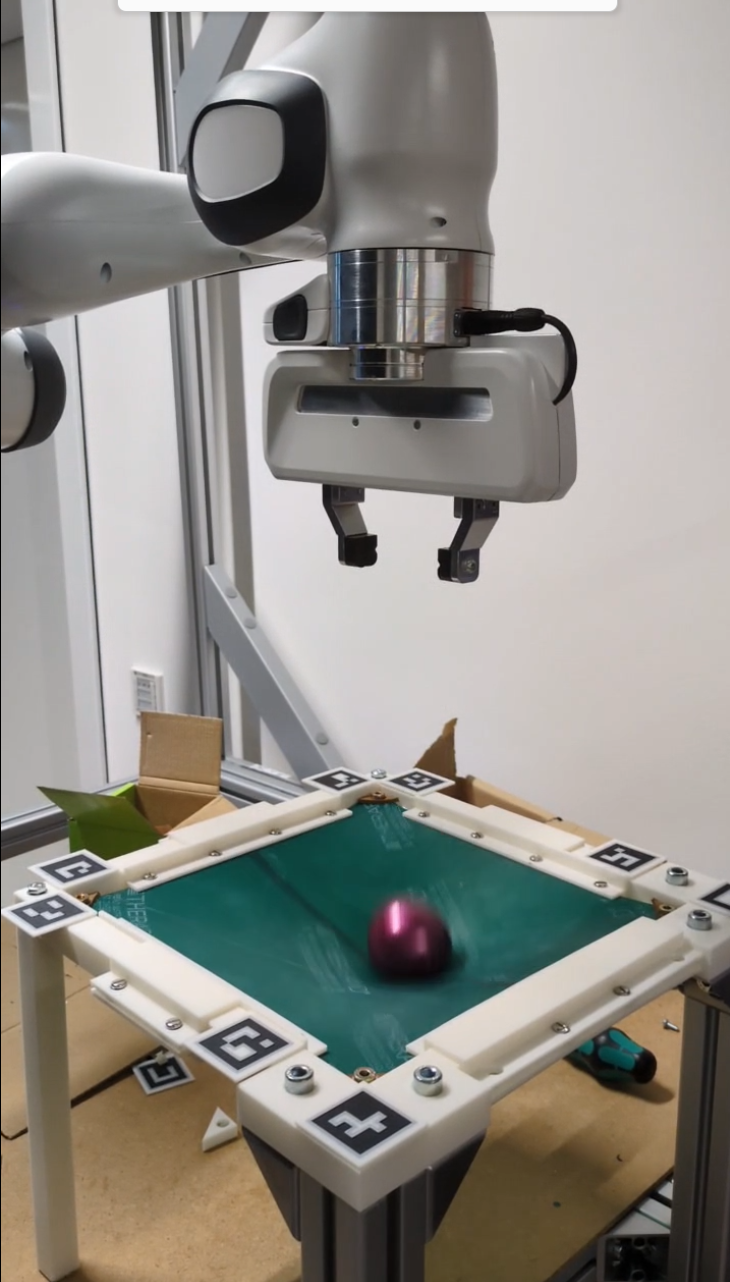
\includegraphics[width=0.192\textwidth, trim={0 2.5cm 0 3.5cm}, clip]{figures/qualitative_realworld_data/03.png}\hfill
  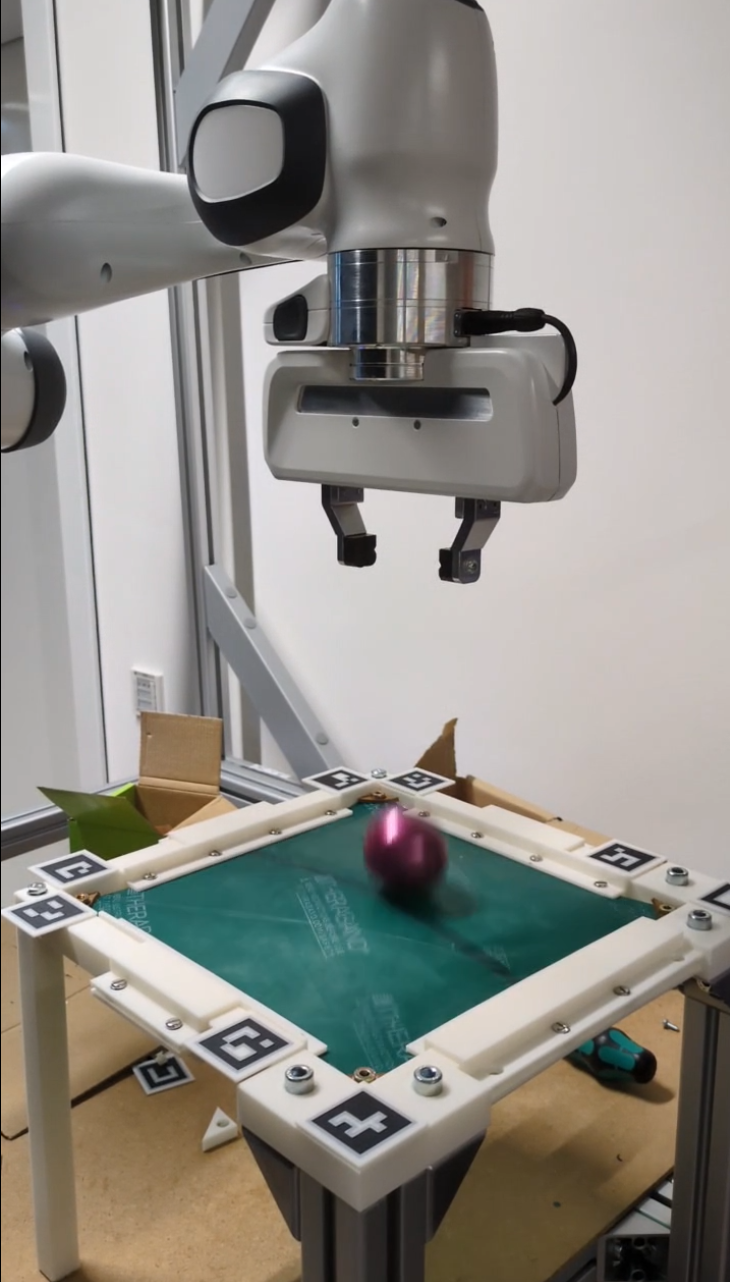
\includegraphics[width=0.192\textwidth, trim={0 2.5cm 0 3.5cm}, clip]{figures/qualitative_realworld_data/04.png}\hfill
  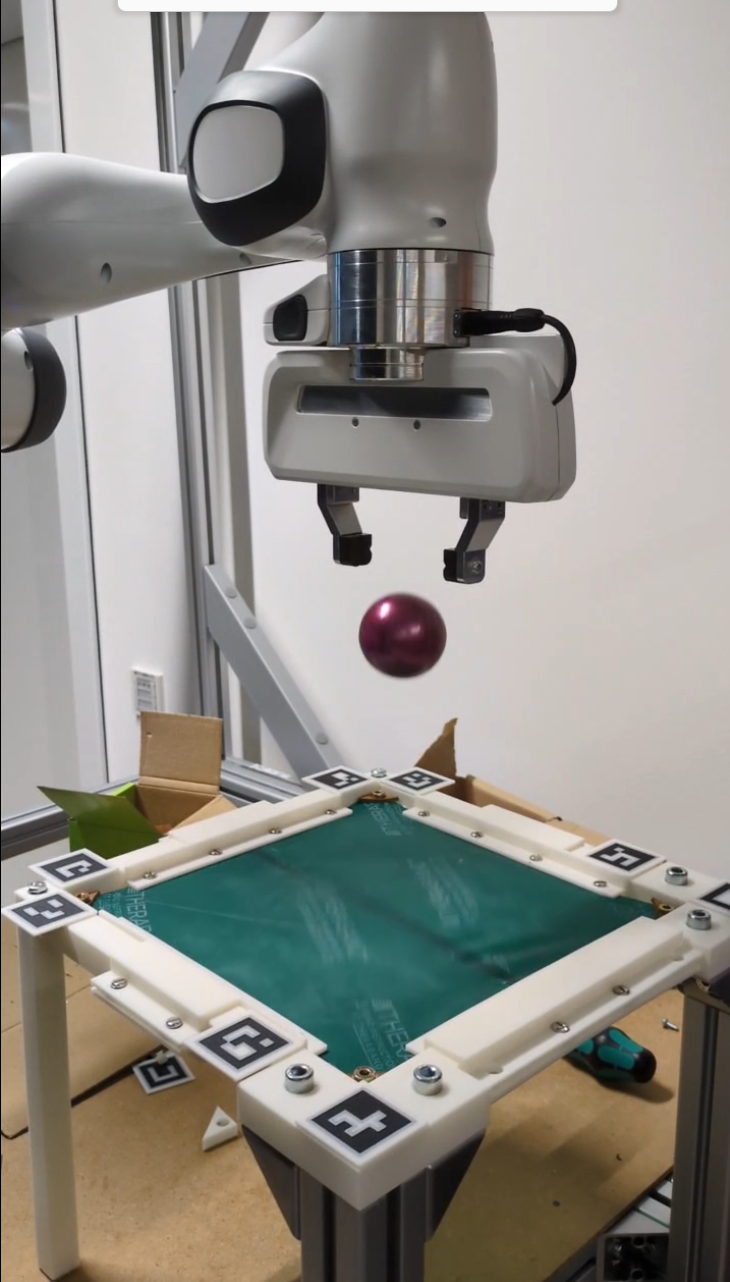
\includegraphics[width=0.192\textwidth, trim={0 2.5cm 0 3.5cm}, clip]{figures/qualitative_realworld_data/05.png}
  \caption{Real-world \texttt{Trampoline} setup. A robot arm releases a steel ball above an elastic membrane stretched across a 3D-printed frame, with ArUco markers at the corners for calibration.}
  \label{fig:realworld_setup}
  \vspace{-0.3cm}
\end{figure}